\section{Why is Lattice Crypto important, interesting,\ldots}
\begin{frame}{Why is Lattice Based Crypto important?}{Or interesting? Or\ldots?}
    \begin{block}{Some facts}
    \begin{itemize}
        \visible<1->{\item It is a Post-Quantum secure Cryptosystem (PQC)}
        \visible<2->{\item It is damn fast (faster than dinosauRS cryptA)}
        \visible<3->{\item You can build anything you want from it:\\
                  Encryption, Signatures, even Hash Functions!}
        \visible<4->{\item It allows to build even one of the most hailed advanced cryptographic building block:\\
                     Fully Homomorphic Encryption (FHC) \includemedia[
                     addresource=data/holygrenade.mp3,
                     flashvars={source=data/holygrenade.mp3
                                &autoplay=true}]{(hallelujah!)}{APlayer.swf}
                    }
    \end{itemize}
    \end{block}
\end{frame}

\section{How does Lattice Crypto work?}
\begin{frame}{How does Lattice Based Crypto work?}{Wait! Lattice, wtf?}
    \visible<1->{%
    \begin{block}{Definition:}
        A lattice $L$ is an discrete, additive, abelian subgroup of $\mathbb{R}^n$.
    \end{block}}
    \visible<2->{%
    \begin{block}{Definition:}
        Let $b_1, b_2, \ldots{}, b_d \in \mathbb{R}^n,\ d \leq n$ linear independent.
        Then the set
        \begin{equation*}
            L = \set{v \in \mathbb{R}^n \given v = \sum_{i=1}^{d} a_i b_i, a_i \in \mathbb{Z}}
        \end{equation*}
        is a lattice.
    \end{block}}
\end{frame}

\begin{frame}{Hey! You promised, this will be easy!}
    \begin{block}{Lattice, dt\@.: Gitter}
        \centering
        \includegraphics[keepaspectratio, width=\textwidth, height=0.5\textheight]{data/gitterkartoffel.jpg}
    \end{block}
\end{frame}

\begin{frame}{Hey! You promised, this will be easy!}{OK, OK, we can say it easier: $\mathbb{Z}^2$ is a Lattice}
    \begin{columns}
        \visible<1->{%
        \begin{column}{0.4\textwidth}
            \begin{block}{\only<1>{Example lattice}\only<2->{Random Basis\vphantom{p}}}
                \centering
                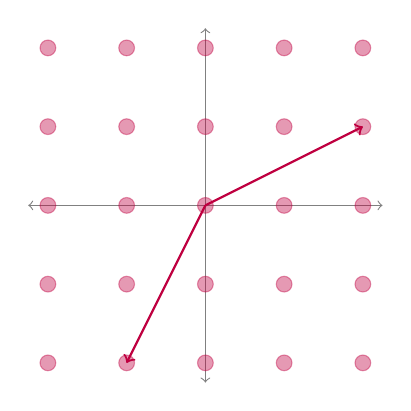
\begin{tikzpicture}
                    \draw [gray] [<->] (-2.25,0) -- (2.25,0);
                    \draw [gray] [<->] (0,-2.25) -- (0,2.25);

                    \foreach \i in {-2, -1, 0, 1, 2}{%
                        \foreach \j in {-2, -1, 0, 1, 2}{%
                            \draw [fill,purple,opacity=.4] (\i,\j) circle [radius=0.1];
                        }
                    }
                    \only<2->{%
                        \draw [thick,purple] [->] (0,0) -- (2, 1);
                        \draw [thick,purple] [->] (0,0) -- (-1, -2);
                    }
                \end{tikzpicture}
            \end{block}
        \end{column}
        }

        \visible<3->{%
        \begin{column}{0.4\textwidth}
            \begin{block}{Reduced Basis\vphantom{p}}
                \centering
                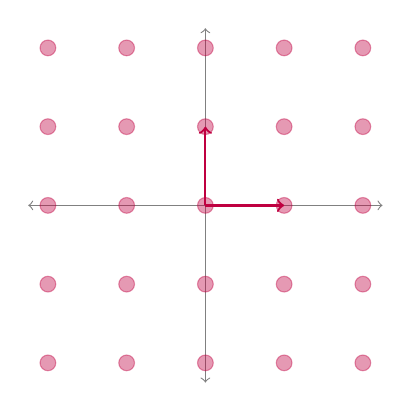
\begin{tikzpicture}
                    \draw [gray] [<->] (-2.25,0) -- (2.25,0);
                    \draw [gray] [<->] (0,-2.25) -- (0,2.25);

                    \foreach \i in {-2, -1, 0, 1, 2}{%
                        \foreach \j in {-2, -1, 0, 1, 2}{%
                            \draw [fill,purple,opacity=.4] (\i,\j) circle [radius=0.1];
                        }
                    }

                    \draw [thick,purple] [->] (0,0) -- (1, 0);
                    \draw [thick,purple] [->] (0,0) -- (0, 1);
                \end{tikzpicture}
            \end{block}
        \end{column}
        }
    \end{columns}
\end{frame}

\begin{frame}{Hard Problems in Lattices\ldots}{\ldots are what we need for crypto.}
    \begin{columns}
        \visible<1->{%
        \begin{column}{0.55\textwidth}
            \begin{block}{Shortest Vector Problem (SVP)}
                Given a lattice $L$, what is the shortest vector $v \in L\setminus \set{\mathbf{0}}$?
            \end{block}
        \end{column}
        }

        \visible<2->{%
        \begin{column}{0.4\textwidth}
            \begin{block}{Example}
                \centering
                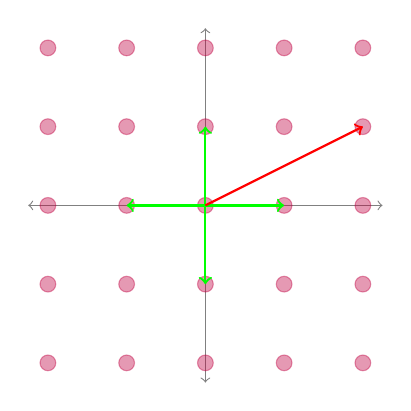
\begin{tikzpicture}
                    \draw [gray] [<->] (-2.25,0) -- (2.25,0);
                    \draw [gray] [<->] (0,-2.25) -- (0,2.25);

                    \foreach \i in {-2, -1, 0, 1, 2}{%
                        \foreach \j in {-2, -1, 0, 1, 2}{%
                            \draw [fill,purple,opacity=.4] (\i,\j) circle [radius=0.1];
                        }
                    }

                    \draw [thick,green] [->] (0,0) -- (1, 0);
                    \draw [thick,green] [->] (0,0) -- (0, 1);
                    \draw [thick,green] [->] (0,0) -- (-1, 0);
                    \draw [thick,green] [->] (0,0) -- (0, -1);
                    \draw [thick,red] [->] (0,0) -- (2, 1);
                \end{tikzpicture}
            \end{block}
        \end{column}
        }
    \end{columns}
\end{frame}

\begin{frame}{Hard Problems in Lattices\ldots}{\ldots are what we need for crypto.}
    \begin{columns}
        \visible<1->{%
        \begin{column}{0.55\textwidth}
            \begin{block}{Closest Vector Problem (CVP)}
                Given a lattice $L$ and a target $t \notin L$, what is the closest vector $v \in L$ to $t$\vphantom{$v \in L\setminus \set{\mathbf{0}}$}?
            \end{block}
        \end{column}
        }

        \visible<2->{%
        \begin{column}{0.4\textwidth}
            \begin{block}{Example}
                \centering
                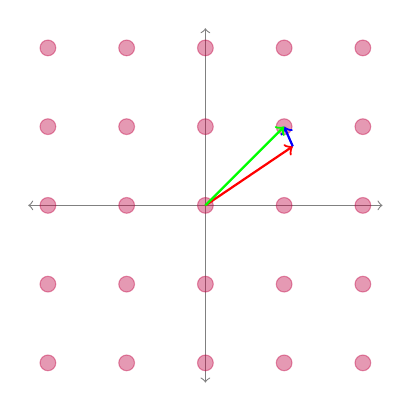
\begin{tikzpicture}
                    \draw [gray] [<->] (-2.25,0) -- (2.25,0);
                    \draw [gray] [<->] (0,-2.25) -- (0,2.25);

                    \foreach \i in {-2, -1, 0, 1, 2}{%
                        \foreach \j in {-2, -1, 0, 1, 2}{%
                            \draw [fill,purple,opacity=.4] (\i,\j) circle [radius=0.1];
                        }
                    }
                    \draw [thick,red] [->] (0,0) -- (1.11, 0.75);
                    \draw [thick,blue] [->] (1.11, 0.75) -- (1, 1);
                    \draw [thick,green] [->] (0,0) -- (1, 1);
                \end{tikzpicture}
            \end{block}
        \end{column}
        }
    \end{columns}
\end{frame}


\begin{frame}{Lattice Based Crypto}
    \begin{block}{Key Generation}
        \centering
        \includegraphics[keepaspectratio,width=\textwidth,height=0.8\textheight]{data/keygen}
    \end{block}
\end{frame}

\begin{frame}{Lattice Based Crypto}
    \begin{block}{Encryption}
        \centering
        \includegraphics[keepaspectratio,width=\textwidth,height=0.8\textheight]{data/encryption}
    \end{block}
\end{frame}

\begin{frame}{Lattice Based Crypto}
    \begin{block}{Decryption}
        \centering
        \includegraphics[keepaspectratio,width=\textwidth,height=0.8\textheight]{data/decryption}
    \end{block}
\end{frame}

\section{Attacks on Lattice Based Crypto}
\begin{frame}{Attack Algorithms}
    \begin{itemize}
        \item Embedding Approach (Kannan)
        \item Enumeration (Babai, Lindner and Peikert, Gamma~\etal/)
    \end{itemize}
\end{frame}

\begin{frame}{Vector Enumeration}
    \only<1>{%
    \begin{block}{Attack}
        \centering
        \includegraphics[keepaspectratio,width=\textwidth,height=0.8\textheight]{data/Eve}
    \end{block}
    }
    \only<2>{%
    \begin{block}{Attack}
        \centering
        \includegraphics[keepaspectratio,width=\textwidth,height=0.8\textheight]{data/attack_step1}
    \end{block}
    }
    \only<3>{%
    \begin{block}{Attack}
        \centering
        \includegraphics[keepaspectratio,width=\textwidth,height=0.8\textheight]{data/attack_step2}
    \end{block}
    }
\end{frame}

\section{OK\@. And what did I do?}
\begin{frame}{Parallel Implementation of BDD enumeration for LWE}
\end{frame}
